%%% Для сборки выполнить 2 раза команду: pdflatex <имя файла>

\documentclass[a4paper,12pt]{article}

\usepackage{ucs}
\usepackage[utf8x]{inputenc}
\usepackage[russian]{babel}
%\usepackage{cmlgc}
\usepackage{graphicx}
\usepackage{listings}
\usepackage{xcolor}
%\usepackage{courier}

\makeatletter
\renewcommand\@biblabel[1]{#1.}
\makeatother

\newcommand{\myrule}[1]{\rule{#1}{0.4pt}}
\newcommand{\sign}[2][~]{{\small\myrule{#2}\\[-0.7em]\makebox[#2]{\it #1}}}

% Поля
\usepackage[top=20mm, left=30mm, right=10mm, bottom=20mm, nohead]{geometry}
\usepackage{indentfirst}

% Межстрочный интервал
\renewcommand{\baselinestretch}{1.50}


\begin{document}

%%%%%%%%%%%%%%%%%%%%%%%%%%%%%%%
%%%                         %%%
%%% Начало титульного листа %%%

\thispagestyle{empty}
\begin{center}
\renewcommand{\baselinestretch}{1}
\large
{\sc Министерство образования и науки Российской Федерации\\
ФГБОУ <<Петрозаводский государственный университет>>\\
Институт математики и информационных технологий\\
Кафедра информатики и математического обеспечения}

\end{center}

\vfill

\begin{center}
{\normalsize Промежуточный отчет о научно-исследовательской работе} \\

\medskip

%%% Название работы %%%
{\Large \sc Мобильное приложение персонализированный трекер пользователя}
\end{center}

\medskip

\begin{flushright}
\parbox{11cm}{%
\renewcommand{\baselinestretch}{1.2}
\normalsize
Выполнил:\\
%%% ФИО студента %%%
студент 2 курса группы 22207 В. В. Клименко
\begin{flushright}
\sign[подпись]{4cm}
\end{flushright}

Научный руководитель:\\
%%% степень, звание ФИО научного руководителя %%%
к.ф.-м.н., преподаватель В. М. Димитров\\
Оценка руководителя:\hfill\rule{4cm}{0.4pt}
\begin{flushright}
\sign[подпись]{4cm}
\end{flushright}

Представлен на кафедру
\begin{flushright}
  <<~\myrule{0.8cm}~>>~\myrule{4cm}~~2018~г.\\[1em]
  \sign[подпись принявшего работу]{6cm}
\end{flushright}
}
\end{flushright}

\vfill

\begin{center}
\large
Петрозаводск --- 2018
\end{center}

%%% Конец титульного листа  %%%
%%%                         %%%
%%%%%%%%%%%%%%%%%%%%%%%%%%%%%%%
\pagebreak
%%%%%%%%%%%%%%%%%%%%%%%%%%%%%%%%
%%%                          %%%
%%% Содержание               %%%

\newpage

\tableofcontents


%%% Содержание              %%%
%%%                         %%%
%%%%%%%%%%%%%%%%%%%%%%%%%%%%%%%

\pagebreak

%%%%%%%%%%%%%%%%%%%%%%%%%%%%%%%%
%%%                          %%%
%%% Введение                 %%%

%%% В введении Вы должны описать предметную область, с которой связана %%%
%%% Ваша работа, показать её актуальность, вкратце определить цель     %%%
%%% исследования/разработки					       %%%

\section*{Введение}
\addcontentsline{toc}{section}{Введение}

Трекер - это программа позволяющая отслеживать путь пользователя и выводить
различную информацию о том, каким образом он перемещался.

Сегодня такое приложение необходимо тем, кто занимается туризмом и спортом.
Ведь это очень удобно, чтобы человек имел статистику о том, с какой скоростью,
где и сколько он прошёл. Однако пользователь вынужден включать и выключать 
запись своих передвижений, что уменьшает удобность использования.
Целью данной работы является создание трекера, котрый работал бы в фоновом режиме,
то есть постоянно вёл запись перемещений без участия пользователя.

\begin{figure}
	\centering
	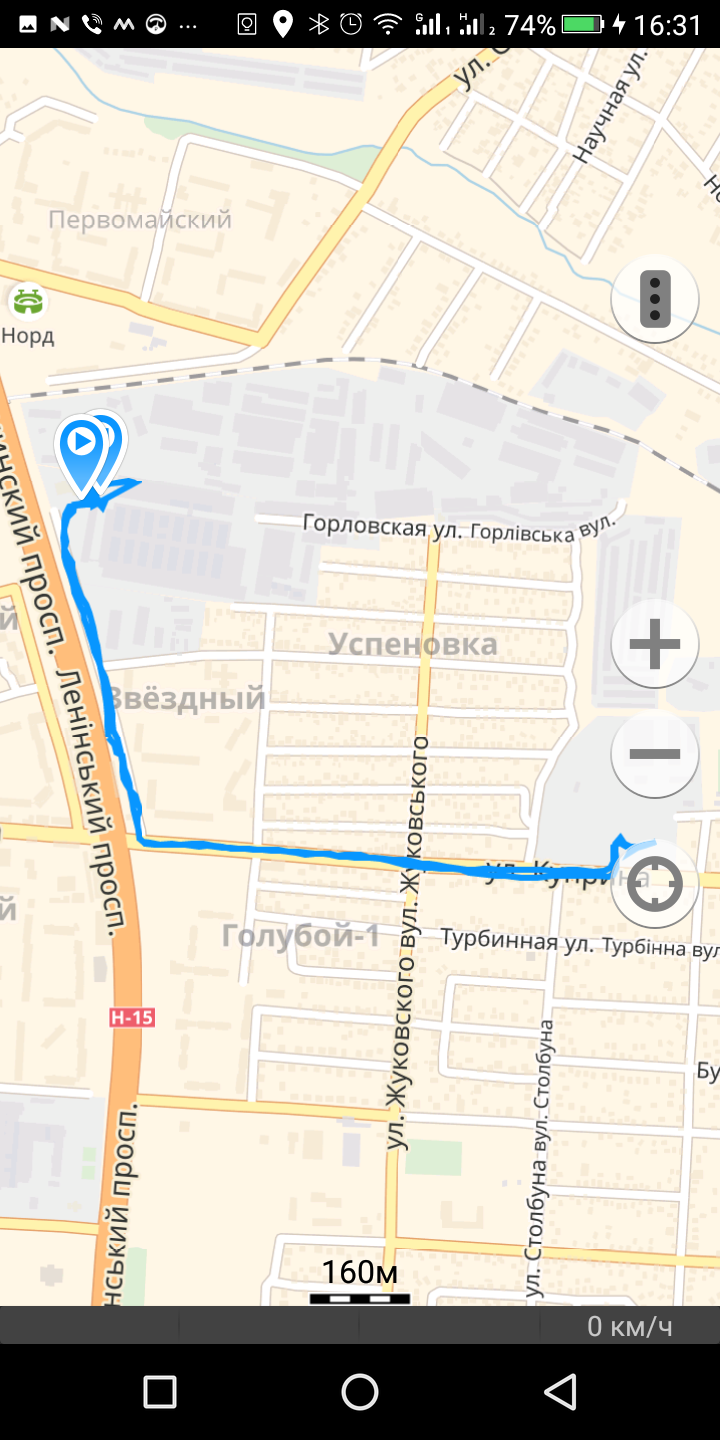
\includegraphics[width=10.94cm]{images/example.png}
	\caption{Пример трекера}
	\label{fig:card}
\end{figure}


%%% Введение                %%%
%%%                         %%%
%%%%%%%%%%%%%%%%%%%%%%%%%%%%%%%

\pagebreak
%%%%%%%%%%%%%%%%%%%%%%%%%%%%%%%%
%%%                          %%%
%%% Обзор                    %%%

%%% В обзоре раскрывается текущее состояние исследований/разработок    %%%
%%% в выбранной Вами области                                           %%%

\section{Разработка тестового приложения}

\subsection{Java-код приложения}

Ниже приведён java-код приложения.

\lstset{ %
	% \usepackage{color} or \usepackage{xcolor}; should come as last argument
	basicstyle=\ttfamily\footnotesize,
	breakatwhitespace=false,
	breaklines=true,
	captionpos=b,
	deletekeywords={...},
	escapeinside={\%*}{*)},
	extendedchars=true,
	keepspaces=true,
	language=C,
	morekeywords={*,...},
	showspaces=false,
	showstringspaces=false,
	showtabs=false,
	numbers=none,
	numbersep=8pt,
	tabsize=4,
	frame=lines,	
	title=\lstname
}


\begin{lstlisting}[caption=Основной код прилжения из LocationActivity.java]
package com.beginerdranch.android.myapplication;


import android.Manifest;
import android.app.Activity;
import android.content.pm.PackageManager;
import android.location.Location;
import android.os.Bundle;
import android.support.v4.app.ActivityCompat;
import android.util.Log;
import android.view.View;
import android.widget.Button;
import android.widget.TextView;

import com.google.android.gms.common.ConnectionResult;
import com.google.android.gms.common.GooglePlayServicesUtil;
import com.google.android.gms.common.api.GoogleApiClient;
import com.google.android.gms.common.api.PendingResult;
import com.google.android.gms.common.api.Status;
import com.google.android.gms.location.LocationListener;
import com.google.android.gms.location.LocationRequest;
import com.google.android.gms.location.LocationServices;

import java.text.DateFormat;
import java.util.Date;

public class LocationActivity extends Activity implements
LocationListener,
GoogleApiClient.ConnectionCallbacks,
GoogleApiClient.OnConnectionFailedListener {

	private static final String TAG = "LocationActivity";
	private static final long INTERVAL = 1000 * 10;
	private static final long FASTEST_INTERVAL = 1000 * 5;
	Button btnFusedLocation;
	TextView tvLocation;
	LocationRequest mLocationRequest;
	GoogleApiClient mGoogleApiClient;
	Location mCurrentLocation;
	String mLastUpdateTime;
	
	protected void createLocationRequest() {
		mLocationRequest = new LocationRequest();
		mLocationRequest.setInterval(INTERVAL);
		mLocationRequest.setFastestInterval(FASTEST_INTERVAL);
		mLocationRequest.setPriority(LocationRequest.PRIORITY_HIGH_ACCURACY);
	}
	
	@Override
	protected void onCreate(Bundle savedInstanceState) {
		super.onCreate(savedInstanceState);
		//show error dialog if GoolglePlayServices not available
		if (!isGooglePlayServicesAvailable()) {
			finish();
		}
		createLocationRequest();
		mGoogleApiClient = new GoogleApiClient.Builder(this)
		.addApi(LocationServices.API)
		.addConnectionCallbacks(this)
		.addOnConnectionFailedListener(this)
		.build();
		
		setContentView(R.layout.activity_location);
		tvLocation = (TextView) findViewById(R.id.tvLocation);
		
		btnFusedLocation = (Button) findViewById(R.id.btnShowLocation);
		btnFusedLocation.setOnClickListener(new View.OnClickListener() {
			@Override
			public void onClick(View arg0) {
				updateUI();
			}
		});	
	}
	
	@Override
	public void onStart() {
		super.onStart();
		mGoogleApiClient.connect();
	}
	
	@Override
	public void onStop() {
		super.onStop();
		mGoogleApiClient.disconnect();
	}
	
	private boolean isGooglePlayServicesAvailable() {
		int status = GooglePlayServicesUtil.isGooglePlayServicesAvailable(this);
		if (ConnectionResult.SUCCESS == status) {
			return true;
		} else {
			GooglePlayServicesUtil.getErrorDialog(status, this, 0).show();
			return false;
		}
	}
	
	@Override
	public void onConnected(Bundle bundle) {
		startLocationUpdates();
	}
	
	protected void startLocationUpdates() {
		if (ActivityCompat.checkSelfPermission(this, 
		Manifest.permission.ACCESS_FINE_LOCATION) != PackageManager.PERMISSION_GRANTED && 
		ActivityCompat.checkSelfPermission(this, 
		Manifest.permission.ACCESS_COARSE_LOCATION) != PackageManager.PERMISSION_GRANTED) {
		// TODO: Consider calling
		//    ActivityCompat#requestPermissions
		// here to request the missing permissions, and then overriding
		//   public void onRequestPermissionsResult(int requestCode, String[] permissions,
		//                                          int[] grantResults)
		// to handle the case where the user grants the permission. See the documentation
		// for ActivityCompat#requestPermissions for more details.
			return;
		}
		PendingResult<Status> pendingResult = LocationServices.FusedLocationApi.requestLocationUpdates(
		mGoogleApiClient, mLocationRequest, this);
	}
	
	@Override
	public void onConnectionSuspended(int i) {
	
	}
	
	@Override
	public void onConnectionFailed(ConnectionResult connectionResult) {
	
	}
	
	@Override
	public void onLocationChanged(Location location) {
		mCurrentLocation = location;
		mLastUpdateTime = DateFormat.getTimeInstance().format(new Date());
		updateUI();
	}
	
	private void updateUI() {
		if (null != mCurrentLocation) {
			String lat = String.valueOf(mCurrentLocation.getLatitude());
			String lng = String.valueOf(mCurrentLocation.getLongitude());
			tvLocation.setText("At Time: " + mLastUpdateTime + "\n" +
			"Latitude: " + lat + "\n" +
			"Longitude: " + lng + "\n" +
			"Accuracy: " + mCurrentLocation.getAccuracy() + "\n" +
			"Provider: " + mCurrentLocation.getProvider());
		} else {
		}
	}
	
	@Override
	protected void onPause() {
		super.onPause();
		stopLocationUpdates();
	}
	
	protected void stopLocationUpdates() {
		LocationServices.FusedLocationApi.removeLocationUpdates(
		mGoogleApiClient, this);
	}
	
	@Override
	public void onResume() {
		super.onResume();
		if (mGoogleApiClient.isConnected()) {
			startLocationUpdates();
		}
	}
}
\end{lstlisting}

\subsection{XML-разметка приложения}

Ниже приведена XML-разметка приложения.

\lstset{ %
	% \usepackage{color} or \usepackage{xcolor}; should come as last argument
	basicstyle=\ttfamily\footnotesize,
	breakatwhitespace=false,
	breaklines=true,
	captionpos=b,
	deletekeywords={...},
	escapeinside={\%*}{*)},
	extendedchars=true,
	keepspaces=true,
	language=C,
	morekeywords={*,...},
	showspaces=false,
	showstringspaces=false,
	showtabs=false,
	numbers=none,
	numbersep=8pt,
	tabsize=4,
	frame=lines,	
	title=\lstname
}


\begin{lstlisting}[caption=Разметка прилжения из activity\_location.xml]
<?xml version="1.0" encoding="utf-8"?>
	<android.support.constraint.ConstraintLayout xmlns:android="http://schemas.android.com/apk/res/android"
		xmlns:app="http://schemas.android.com/apk/res-auto"
		xmlns:tools="http://schemas.android.com/tools"
		android:layout_width="match_parent"
		android:layout_height="match_parent"
		tools:context=".LocationActivity">
	
	<TextView
		android:id="@+id/textView"
		android:layout_width="wrap_content"
		android:layout_height="wrap_content"
		android:layout_centerHorizontal="true"
		android:layout_marginTop="45dp"
		android:text="@string/locationTxt"
		app:layout_constraintStart_toStartOf="parent"
		app:layout_constraintTop_toTopOf="parent" />
	
	<Button
		android:id="@+id/btnShowLocation"
		style="?android:attr/buttonStyleSmall"
		android:layout_width="fill_parent"
		android:layout_height="wrap_content"
		android:layout_below="@+id/textView"
		android:layout_centerHorizontal="true"
		android:layout_marginTop="270dp"
		android:background="#ffff1a7c"
		android:text="Show Location"
		android:textColor="#ffffffff"
		app:layout_constraintStart_toStartOf="parent"
		app:layout_constraintTop_toBottomOf="@+id/tvLocation" />
	
	<TextView
		android:id="@+id/tvLocation"
		android:layout_width="fill_parent"
		android:layout_height="wrap_content"
		android:layout_alignParentBottom="true"
		android:layout_marginTop="18dp"
		app:layout_constraintStart_toStartOf="parent"
		app:layout_constraintTop_toBottomOf="@+id/textView" />
</android.support.constraint.ConstraintLayout>
\end{lstlisting}


\begin{figure}
	\centering
	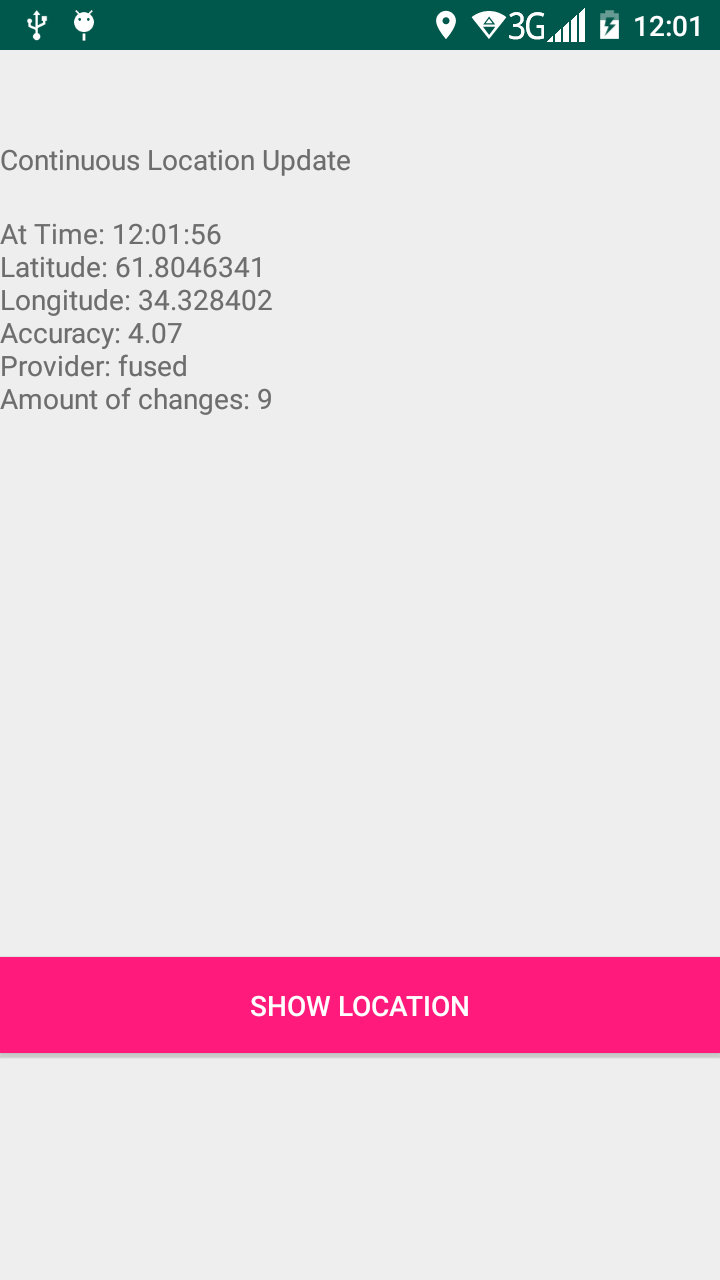
\includegraphics[width=10.94cm]{images/Screenshot_2018-12-07-12-01-59.png}
	\caption{Внешний вид тестового приложения при работе}
	\label{fig:card}
\end{figure}


%%% Обзор                   %%%
%%%                         %%%
%%%%%%%%%%%%%%%%%%%%%%%%%%%%%%%

\pagebreak
%%%%%%%%%%%%%%%%%%%%%%%%%%%%%%%%
%%%                          %%%
%%% Постановка задачи        %%%

%%% Итогом этого раздела должна быть ясная формулировка задач, требующих %%%
%%% решения для достижения цели, кратко указанной во введении            %%%

\section{Постановка задачи}

\subsection{Создание трекера пользователя}

Такая серьёзная задача требует знаний и умений в области
разработки приложений под платформу Android. Прежде всего
требуется разработать тестовый вариант приложения, который
позволит оценить расход батареи мобильного устройства. Оно
постоянно работать и опрашивать местоположение пользователя.
Статистика расхода батареи позволит сделать вывод
о возможности создания энергоэффективного трекера.

Для достижения поставленной цели необходимо решить задачи:

\begin{enumerate}
\item Изучить основные принципы разработки мобильного приложения
\item Установить и настроить инструменты разрабодки под платформу Android
\item Изучить основные технологии создания приложений под платформу Android
\item Изучить технологии отслеживания местоположения
\item Изучить технологии работы приложения в фоновом режиме
\item Написать тестовое приложение
\item Написать основное приложение
\end{enumerate}

%%% Постановка задачи        %%%
%%%                          %%%
%%%%%%%%%%%%%%%%%%%%%%%%%%%%%%%%

\pagebreak
%%%%%%%%%%%%%%%%%%%%%%%%%%%%%%%%
%%%                          %%%
%%% Результаты               %%%

%%% Здесь опишите то, что уже сделано на данном этапе %%%

\section{Текущие результаты}

На данный момент получены следдующие результаты:

\begin{enumerate}
\item Изучены базовые принципы разработки мобильных приложений
\item Установлены и настроены инструменты разработки под Android
\item Изучены основные технологии разработки под платформу Android
\item Изучены технологии отслеживания местоположения
\item Написано тестовое приложение без работы в фоне
\end{enumerate}


%%% Пример внутристрочной и выключной формулы %%%


%%% Результаты               %%%
%%%                          %%%
%%%%%%%%%%%%%%%%%%%%%%%%%%%%%%%%


\pagebreak
%%%%%%%%%%%%%%%%%%%%%%%%%%%%%%%%
%%%                          %%%
%%% Использованные источники %%%

\renewcommand{\bibname}{Библиографический список использованной литературы}
\begin{thebibliography}{99}
%\thispagestyle{empty}
\vspace{5mm}
\addcontentsline{toc}{section}{Библиографический список использованной литературы}

\bibitem{review}
Геотрекер - GPS трекер - Всё о пройденном пути [Электронный ресурс] : [сайт] - Электрон. дан. 
- Режим доступа:http://helpix.ru/appinion/201806/2160-geotreker\_-\_gps\_treker-vsjo\_o\_projdennom\_puti.html - Загл. с экрана.

\bibitem{documentation}
Android Developers [Электронный ресурс] : [сайт] - Электрон. дан. 
- Режим доступа:https://developer.android.com/ - Загл. с экрана.

\bibitem{book}
Филлипс Б., Стюарт К., Марсианко К. {\it Android программирование для профессионалов} М.: Питер. 2017 --- 687 с.

\end{thebibliography}

%%%                          %%%
%%%%%%%%%%%%%%%%%%%%%%%%%%%%%%%%

\end{document}
